\subsection{Figures and Tables}
% \begin{frame}[c,plain,noframenumbering]
% \begin{tikzpicture}[remember picture,overlay]
% \fill[fill=kul-blue]
%     (current page.south east)  rectangle  ([shift={(0,-0.1\paperheight)}]current page.north west)   ;
% \end{tikzpicture}
% \centering
% \vfill
% \textcolor{white}{\Large\textbf{Figures, Tables, Equations, \\\vspace{0.3cm}Algorithms and Listings}}
% \end{frame}

% \begin{frame}[c,plain,noframenumbering]
% \begin{tikzpicture}[remember picture,overlay]
% \fill[fill=gray]
%     (current page.south east)  rectangle ([shift={(0,-0.1\paperheight)}]current page.north west)   ;
% \end{tikzpicture}
% \centering
% \vfill
% \textcolor{white}{\Large\textbf{Figures}}
% \end{frame}


\begin{frame}[fragile]{Including a Figure}
\vspace{.5cm}
	\begin{columns}[t]
		\begin{column}{.5\textwidth}
			Need graphicx package
			\\\quad \pack{graphicx}
			\vskip.05\textheight
			Define a figure environment
			\begin{itemize}
			\item[] \env{figure}{placing specifier}{
			\\\quad \commo{centering}
			\\\quad \commop{includegraphics}{options}{\\pathToFigure}
			\\\quad \comm{caption}{text explaining\\ the figure}\\
			}
			\end{itemize}
		\end{column}
		\begin{column}{.5\textwidth}
			[placing specifier]
			\begin{itemize}
				\item h = here
				\item t = top of the page
				\item b = bottom of the page
				\item p = on a special page for \textit{figures}, \textit{tables}, \textit{etc.}
				\item ! = override LaTeX parameters that normally decide good positioning
			\end{itemize}
		\end{column}
	\end{columns}	
\end{frame}

\begin{frame}[fragile]{Including a Figure}
\vspace{.5cm}
	\begin{columns}[t]
		\begin{column}{.5\textwidth}
			Need graphicx package
			\\\quad \pack{graphicx}
			\vskip.05\textheight
			Define a figure environment
			\begin{itemize}
			\item[] \env{figure}{placing specifier}{
			\\\quad \commo{centering}
			\\\quad \commop{includegraphics}{options}{\\pathToFigure}
			\\\quad \comm{caption}{text explaining\\ the figure}\\
			}
			\end{itemize}
		\end{column}
		\begin{column}{.5\textwidth}
			\commo{centering} makes sure the included figure is centered in the environment
			\vskip.05\textheight
			similar placing as in figures, but now with respect to the other subfigures.
		\end{column}
	\end{columns}	
\end{frame}

\begin{frame}[fragile]{Using Subfigures}
\vspace{.5cm}
	\begin{columns}[t]
		\begin{column}{.5\textwidth}
			Needs
			\\\quad \pack{caption}
                \\\quad \pack{subcaption}
			\vskip.05\textheight
			Define a figure environment
			\begin{itemize}
			\item[] \env{figure}{placing specifier}{
                \\ \quad \env{subfigure}{placing specifier}{
                \\\qquad \commo{includegrpahics}}\\
                \commo{hfill}
                 \\ \quad \env{subfigure}{placing specifier}{
                \\}\\
			}\\
			\end{itemize}
		\end{column}
		\begin{column}{.5\textwidth}
			\commo{subfigure} allows to place different subfigures in one figure environment.
			\vskip.05\textheight
			\commo{includegraphics} finds and inserts the actual figure file
			\begin{itemize}
				\item optional typically refers to the \\width or height of the figure
				\item most often related to \commo{textwidth}, e.g. \texttt{[width=0.5\commo{textwidth}]}
			\end{itemize}
		\end{column}
	\end{columns}	
\end{frame}

% \begin{frame}[fragile]{Including a Figure}
% %\vspace{.5cm}
% 	\begin{columns}[t]
% 		\begin{column}{.5\textwidth}
% 			\begin{figure}
% 			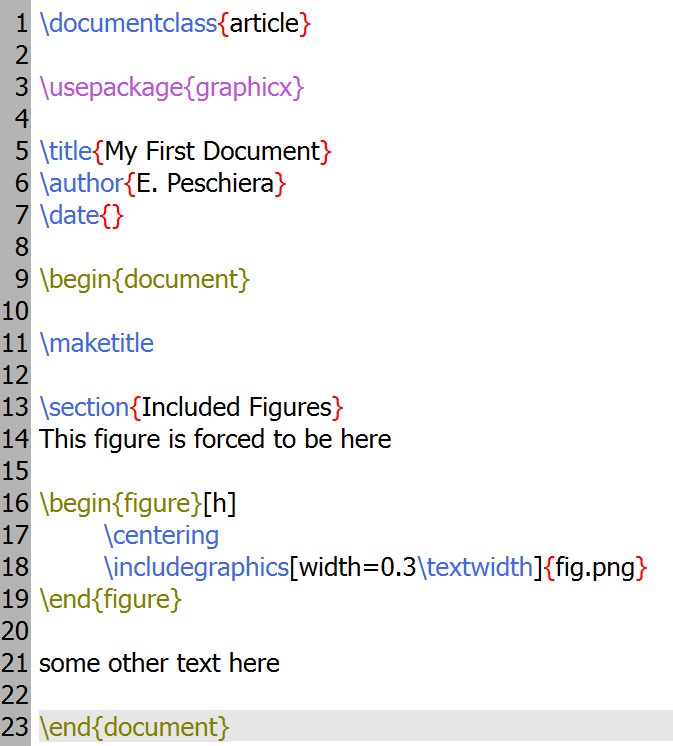
\includegraphics[scale=.45]{Figures/code2}
% 			\end{figure}
% 		\end{column}
% 		\begin{column}{.5\textwidth}
% 			\begin{figure}
% 			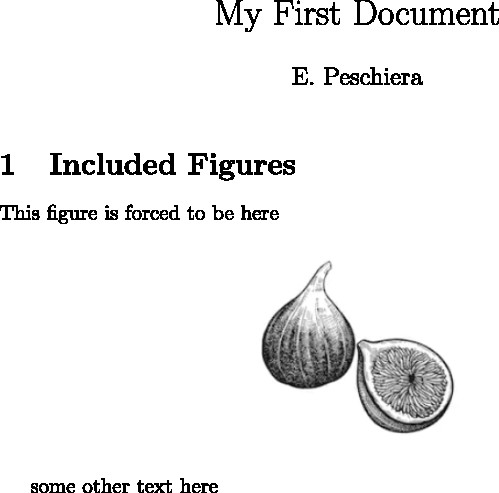
\includegraphics[width=.72\linewidth, frame, trim={-1cm -1cm -1cm -1cm},clip]{Figures/doc3}
% 			\end{figure}
% 		\end{column}
% 	\end{columns}	
% \end{frame}

% \begin{frame}[c,plain,noframenumbering]
% \begin{tikzpicture}[remember picture,overlay]
% \fill[fill=gray]
%     (current page.south east)  rectangle ([shift={(0,-0.1\paperheight)}]current page.north west)   ;
% \end{tikzpicture}
% \centering
% \vfill
% \textcolor{white}{\Large\textbf{Tables}}
% \end{frame}

\begin{frame}[fragile]{Inserting a Table}
\vspace{.5cm}
	\begin{columns}[t]
		\begin{column}{.5\textwidth}
			\env{table}{placing options}{\begin{itemize}
			\item[] \comm{caption}{text explaining the Table}
			\\ \commo{centering}
			\envt{tabular}{columnFormat}{
			\\\quad colTitle \textcolor{red}{\&} \textless repeat for all columns\textgreater \textcolor{blue}{ \textbackslash\textbackslash}
			\\\quad \commo{hline}
			\\\quad data \textcolor{red}{\&} data \textcolor{red}{\&} \textless repeat\textgreater   \textcolor{blue}{ \textbackslash\textbackslash}
			\\\quad \commo{hline}\\}
			\end{itemize}
			}
		\end{column}
		\begin{column}{.5\textwidth}
			\texttt{\textcolor{olive}{table}} environment makes sure that\\ the table can be correctly placed
			\vskip.05\textheight
			\texttt{\textcolor{olive}{tabular}} environment \\= actual table
		\end{column}
	\end{columns}	
\end{frame}

\begin{frame}[fragile]{Inserting a Table}
\vspace{.5cm}
	\begin{columns}[t]
		\begin{column}{.5\textwidth}
			\env{table}{placing options}{\begin{itemize}
			\item[] \comm{caption}{text explaining the Table}
			\\ \commo{centering}
			\envt{tabular}{columnFormat}{
			\\\quad colTitle \textcolor{red}{\&} \textless repeat for all columns\textgreater \textcolor{blue}{ \textbackslash\textbackslash}
			\\\quad \commo{hline}
			\\\quad data \textcolor{red}{\&} data \textcolor{red}{\&} \textless repeat\textgreater   \textcolor{blue}{ \textbackslash\textbackslash}
			\\\quad \commo{hline}\\}
			\end{itemize}
			}
		\end{column}
		\begin{column}{.5\textwidth}
			\texttt{\textcolor{red}{\{}columnFormat\textcolor{red}{\}}} defines
			\begin{itemize}
				\item How many columns in the table
				\item The layout of the columns
				\begin{itemize}
					\item c: centered text
					\item l: left-aligned text
					\item r: right-aligned text
                        \item fixed-width columns \texttt{p\{2cm\}}
                        \begin{itemize}
                            \item m: middle
                            \item p: top
                            \item b: bottom
                        \end{itemize}
				\end{itemize}
				% \item When to draw vertical lines, defined by \textbar
			\end{itemize}
		\end{column}
	\end{columns}	
\end{frame}

\begin{frame}[fragile]{Inserting a Table}
\vspace{.5cm}
	\begin{columns}[t]
		\begin{column}{.5\textwidth}
			\env{table}{placing options}{
			\begin{itemize}
			\item[] \comm{caption}{text explaining the Table}
			\\ \commo{centering}
			\envt{tabular}{columnFormat}{
			\\\quad colTitle \textcolor{red}{\&} \textless repeat for all columns\textgreater \textcolor{blue}{ \textbackslash\textbackslash}
			\\\quad \commo{hline}
			\\\quad data \textcolor{red}{\&} data \textcolor{red}{\&} \textless repeat\textgreater   \textcolor{blue}{ \textbackslash\textbackslash}
			\\\quad \commo{hline}\\}
			\end{itemize}
			}
		\end{column}
		\begin{column}{.5\textwidth}
			\texttt{\textcolor{red}{\&}} is a column separator. Used to show in which column the next \textit{item} goes
			\vskip.05\textheight
			\commo{hline} inserts a horizontal line
			\vskip.05\textheight
			\commo{\textbackslash} is the standard LaTeX command for\\ a line break
			\\\quad In a table: next row
		\end{column}
	\end{columns}	
\end{frame}

\begin{frame}[fragile]{Inserting a Table}
%\vspace{.5cm}
	\begin{columns}[t]
		\begin{column}{.5\textwidth}
			\begin{figure}
			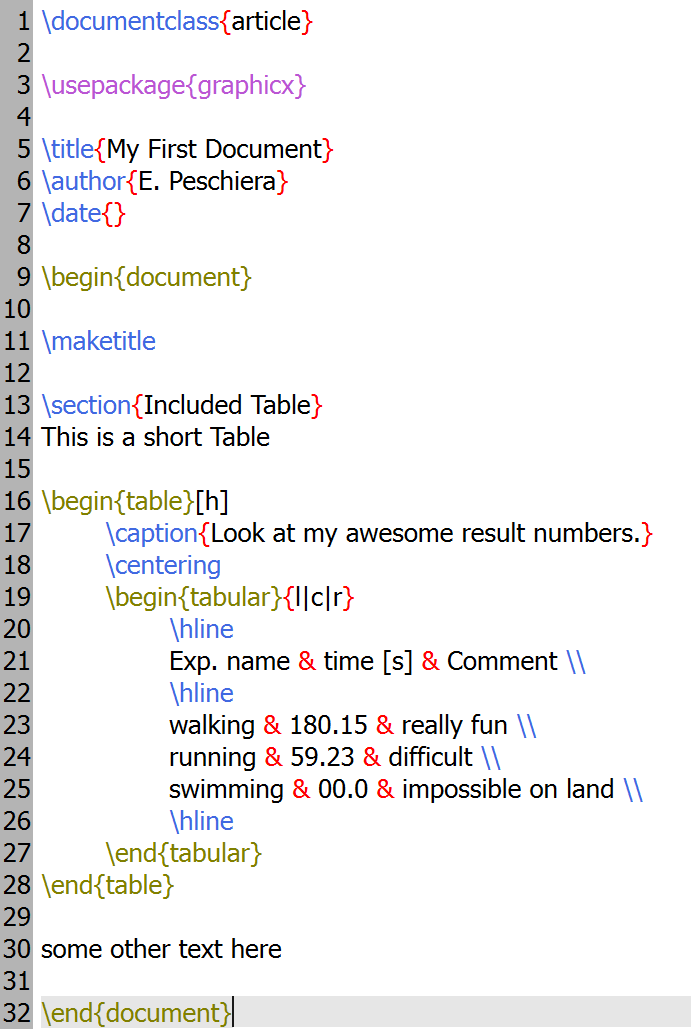
\includegraphics[scale=.35]{Figures/code3}
			\end{figure}
		\end{column}
		\begin{column}{.5\textwidth}
			\begin{figure}
			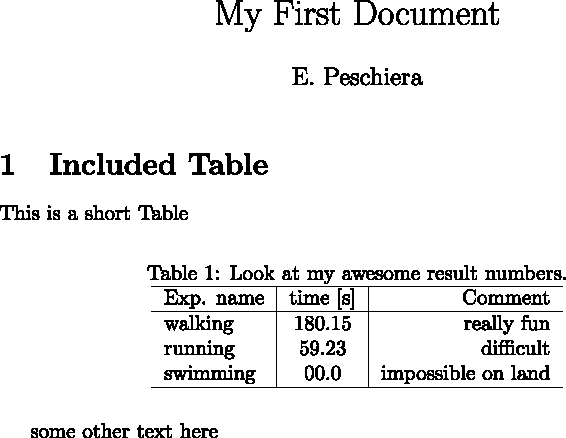
\includegraphics[width=.85\linewidth, frame, trim={-1cm -1cm -1cm -1cm},clip]{Figures/doc4}
			\end{figure}
		\end{column}
	\end{columns}	
\end{frame}

\begin{frame}[fragile]{Note on Figures and Tables}
\vspace{.5cm}
	In case your document is multicolumn, e.g., IEEE paper, but your figure needs to\\ span more than 1 column:
	use * when defining the environment
	\vskip.02\textheight
	\begin{itemize}
		\item[] \envs{figure*}{...}
%		\vskip.01\textheight
		\item[] \envs{table*}{...}
	\end{itemize}
\end{frame}


\begin{frame}[fragile]{Making beautiful tables}
	Highly recommended document: \url{https://people.inf.ethz.ch/markusp/teaching/guides/guide-tables.pdf}.
	\somespace
    Guidelines
	\begin{itemize}
		\item avoid vertical lines
        \item Avoid “boxing up” cells, usually 3 horizontal lines are
enough: above, below, and after heading (see examples in
this guide)
\item avoid double horizontal lines
\item enough space between rows
\item if in doubt, align left
\item right-align numbers (using same notation/unit)
        \item use \pack{booktabs}
	\end{itemize}
\end{frame}


\begin{frame}[fragile]{Making beautiful tables}

\newcommand{\ra}[1]{\renewcommand{\arraystretch}{#1}}
\centering
\resizebox{\textwidth}{!}{%
\ra{1.3}
\setlength\dashlinedash{0.2pt}
\setlength\dashlinegap{1.5pt}
\setlength\arrayrulewidth{0.3pt}

% \begin{tabular}{@{}rrrrcrrrcrrr@{}}\toprule
% & \multicolumn{3}{c}{$w = 8$} & \phantom{abc}& \multicolumn{3}{c}{$w = 16$} &
% \phantom{abc} & \multicolumn{3}{c}{$w = 32$}\\
% \cmidrule{2-4} \cmidrule{6-8} \cmidrule{10-12}
% & $t=0$ & $t=1$ & $t=2$ && $t=0$ & $t=1$ & $t=2$ && $t=0$ & $t=1$ & $t=2$\\ \midrule
% $dir=1$\\
% $c$ & 0.0790 & 0.1692 & 0.2945 && 0.3670 & 0.7187 & 3.1815 && -1.0032 & -1.7104 & -21.7969\\
% $c$ & -0.8651& 50.0476& 5.9384&& -9.0714& 297.0923& 46.2143&& 4.3590& 34.5809& 76.9167\\
% $c$ & 124.2756& -50.9612& -14.2721&& 128.2265& -630.5455& -381.0930&& -121.0518& -137.1210& -220.2500\\
% $dir=0$\\
% $c$ & 0.0357& 1.2473& 0.2119&& 0.3593& -0.2755& 2.1764&& -1.2998& -3.8202& -1.2784\\
% $c$ & -17.9048& -37.1111& 8.8591&& -30.7381& -9.5952& -3.0000&& -11.1631& -5.7108& -15.6728\\
% $c$ & 105.5518& 232.1160& -94.7351&& 100.2497& 141.2778& -259.7326&& 52.5745& 10.1098& -140.2130\\
% \bottomrule
% \end{tabular}

\begin{tabular}{@{}lllrrr@{}}\toprule
\textbf{Rank} & \textbf{Lead Arranger} & \textbf{Number of Deals} & \textbf{Dollar Amount} & \textbf{Market Share} & \textbf{Equator Principles Adoption}\\ \midrule
\textbf{1} & State Bank of India & 52 & \$21,631.6 & 10.1\% & NA\\ \hdashline
\textbf{2} & Mitsubishi UFJ Financial & 88 & 9,486.1 & 4.4 & Dec 2005\\ \hdashline
\textbf{3} & Sumitomo Mitsui & 71 & 8,188.1 & 3.8 & Jan 2006\\ \hdashline
\textbf{4} & Credit Agrocole & 60 & 6,506.4 & 3.1 & Jun 2005\\ \hdashline
\textbf{5} & Mizuho Financial & 55 & 5,797.5 & 2.7 & Oct 2003\\ \hdashline
\textbf{6} & Soci\'{e}t\'{e} Generale & 55 & 5,760.5 & 2.7 & Sep 2007\\ \hdashline
\textbf{7} & BNP Paribas & 55 & 5,390.8 & 2.5 & Oct 2008\\ \hdashline
\textbf{8} & Axis Bank & 18 & 5,216.9 & 2.4 & NA\\ \hdashline
\textbf{9} & IDBI Bank & 10 & 5,162.3 & 2.4 & NA\\ \hdashline
\textbf{10} & ING & 49 & 4,916.1 & 2.3 & Jun 2003\\ \midrule
 & Others & 102 & 135,430.4 & 63.6 & \\ \midrule
 & Total Market & 615 & \$213,486.7 & 100\% & \\
\bottomrule
\end{tabular}
}
\end{frame}
